\documentclass[12pt,a4paper]{article}

\usepackage{fontspec}
\usepackage{polyglossia}
\setdefaultlanguage{russian}
\setotherlanguage{english}
\setmainfont{Times New Roman}
\usepackage{amsmath,amssymb}
\usepackage{graphicx}
\usepackage{booktabs}
\usepackage{geometry}
\usepackage{float}
\usepackage{setspace}

\geometry{left=25mm,right=20mm,top=20mm,bottom=20mm}
\graphicspath{{./}}
\onehalfspacing

\begin{document}

\begin{titlepage}
\begin{center}
\large Отчет по физике\\[1.5cm]
\Large\textbf{Лабораторная работа № 1}\\[0.4cm]
\large Метод конечных разностей\\[2cm]
\end{center}

\begin{flushright}
Выполнил: Панасик Владислав\\[0.5cm]
Группа: 2Б\\[0.5cm]
Проверил: \underline{\hspace{5cm}}
\end{flushright}

\vfill
\begin{center}
2026
\end{center}
\end{titlepage}

\section{Цель работы}
Изучить метод конечных разностей (МКР) на одномерных и двумерных задачах,
построить численные решения, сравнить их с аналитическими решениями там,
где это возможно, и исследовать производные и погрешности. Вычисления и
графики выполнены на Python; файл программы прилагается к отчету отдельно.

\section{Задание 1: уравнение с постоянной правой частью}
\subsection{Выбор параметров и разностная схема}
Для решения задачи выберем \(A=2\), \(B=3\), \(C=1\),
\(D=3.14\) и отрезок \(x\in[0,1]\). Используем 50 узлов
\(x_i=ih\), \(i=0,\ldots,49\), с шагом \(h=1/50=0.02\).
Исходная задача имеет вид
\[
A U''(x)=B,\qquad U(0)=C,\qquad U'(0)=D.
\]
Для внутренних узлов используем центральную разность для второй производной,
а начальную производную аппроксимируем прямой разностью, как в методических
указаниях:
\[
\frac{U_{i+1}-2U_i+U_{i-1}}{h^2}=\frac BA,\qquad
U_0=C,\qquad \frac{U_1-U_0}{h}=D.
\]
Отсюда \(U_1=C+Dh\), а для \(i=1,\ldots,48\)
\[
U_{i+1}=2U_i-U_{i-1}+\frac BA h^2.
\]
В последнем узле \(x_{49}=0.98\) численное значение равно
\(U_{49}\approx4.7828\).

\subsection{Аналитическое решение и погрешность}
Интегрируя исходное уравнение и используя начальные условия, получаем
\[
U_{\text{точн}}(x)=C+Dx+\frac{B}{2A}x^2
=1+3.14x+0.75x^2.
\]
В узле \(x_i\) абсолютное отклонение и относительная погрешность определялись как
\[
\Delta U_i=|U_i-U_{\text{точн}}(x_i)|,\qquad
\varepsilon_i=\frac{\Delta U_i}{|U_{\text{точн}}(x_i)|}\,100\%.
\]
Максимальное абсолютное отклонение на сетке равно \(0.0147\), а максимальная
относительная погрешность --- \(0.3064\%\). В этой схеме ошибка в узле \(i\) равна
\[
U_i-U_{\text{точн}}(x_i)=-i\,\frac{B}{2A}h^2;
\]
она линейно накапливается из-за начального условия разностной схемы
\(U_1=C+Dh\), в котором отсутствует квадратичная поправка точного решения.

\begin{figure}[H]
\centering
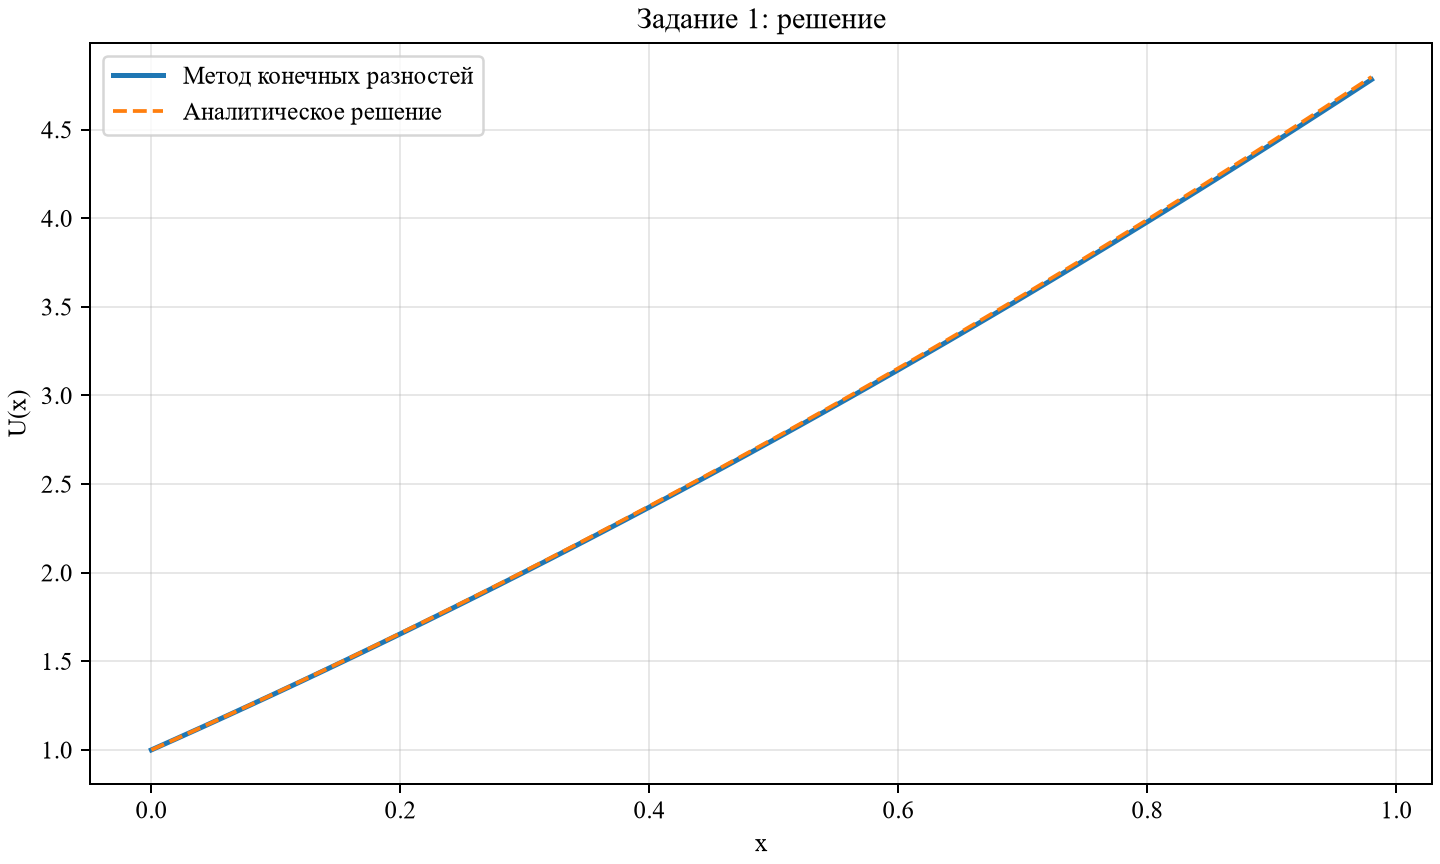
\includegraphics[width=0.78\textwidth]{task1_solution.png}
\caption{Численное и аналитическое решения задачи 1}
\end{figure}
\begin{figure}[H]
\centering
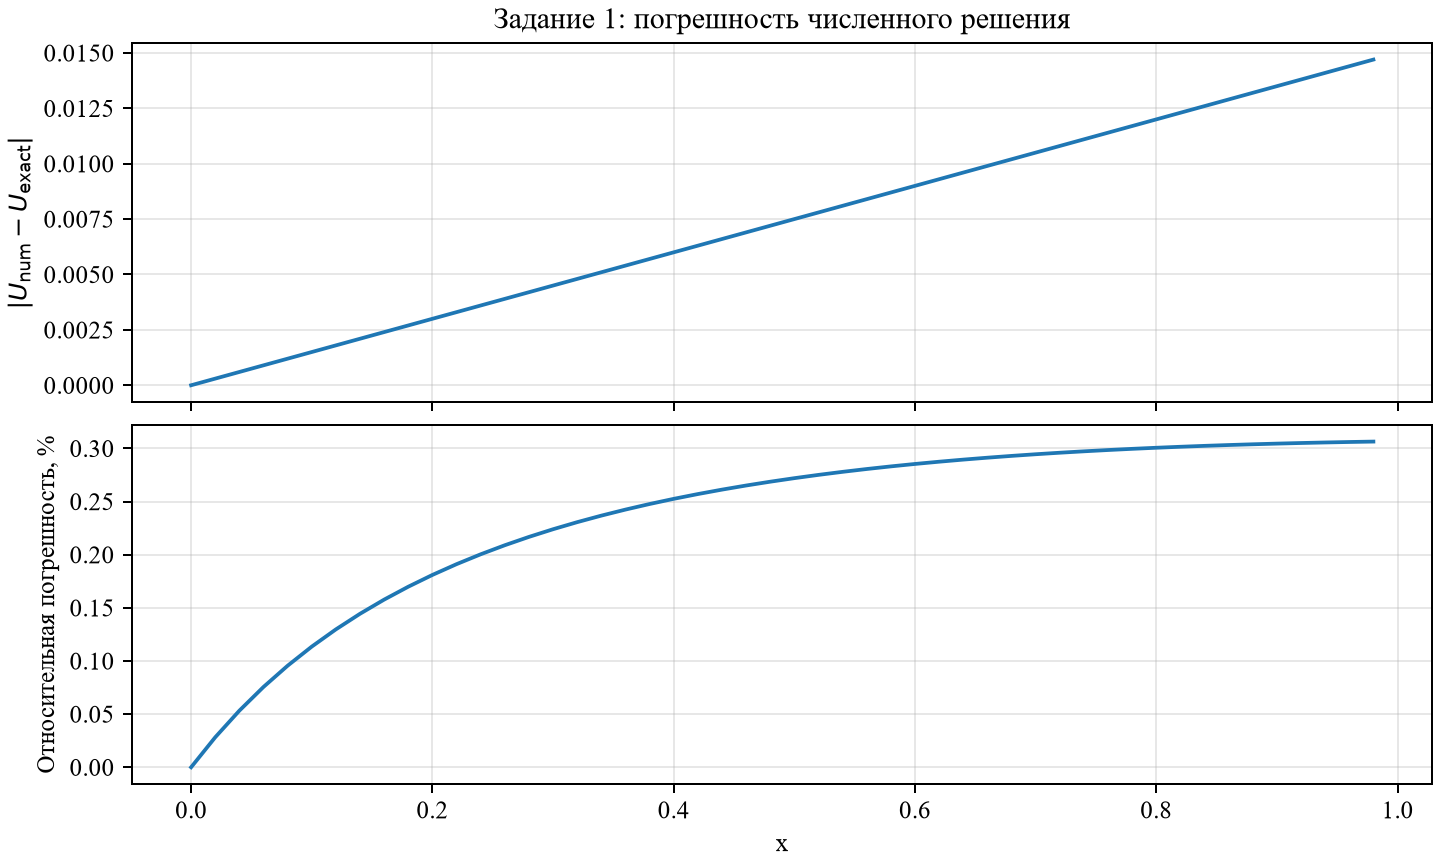
\includegraphics[width=0.82\textwidth]{task1_error.png}
\caption{Абсолютное отклонение и относительная погрешность задачи 1}
\end{figure}

\subsection{Ответы на вопросы к заданию 1}
\paragraph{Что описывает уравнение и какой смысл имеет \(U(x)\)?}
Уравнение \(A U''=B\) описывает одномерное поле с постоянной плотностью
источников (например, потенциал в одномерной модели с постоянным зарядом)
или движение точки под действием постоянной силы, если независимую переменную
трактовать как время, а \(U\) --- как координату. В общем случае \(U(x)\)
задает величину поля/координату, \(U'(x)\) --- ее скорость изменения, а
\(U''(x)=B/A=1.5\) --- постоянную кривизну поля или ускорение.
\paragraph{Какой смысл имеют производные \(U'(x)\) и \(U''(x)\)?}
Первая производная характеризует скорость изменения \(U\) по \(x\), а вторая
--- изменение этой скорости (или кривизну графика).
\[
U'(x)=3.14+1.5x,\qquad U''(x)=1.5.
\]
\begin{figure}[H]
\centering
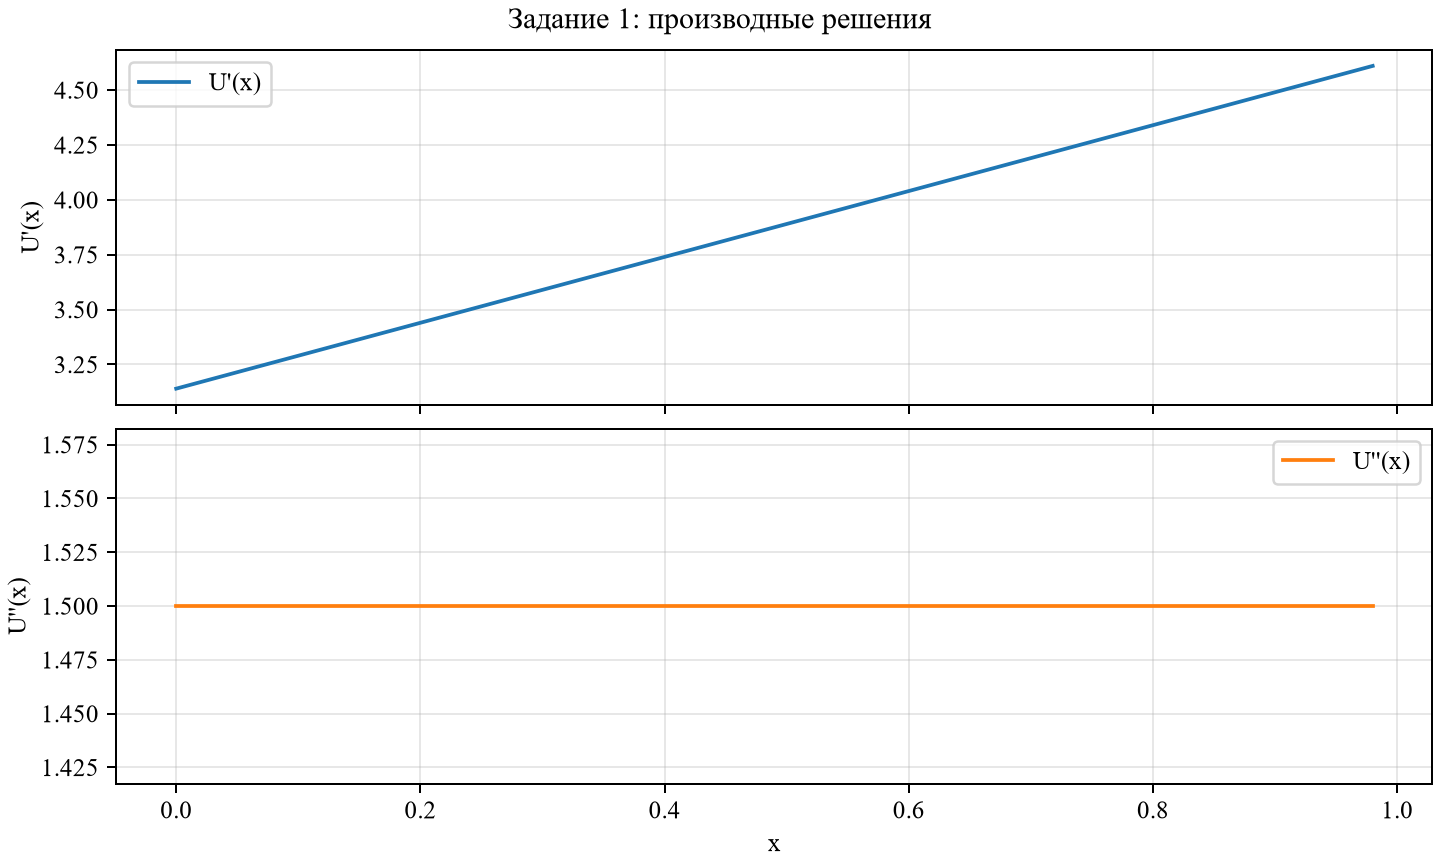
\includegraphics[width=0.75\textwidth]{task1_derivatives.png}
\caption{Первая и вторая производные аналитического решения задачи 1}
\end{figure}

\section{Задание 2: движение}
\subsection{Разностное решение}
Примем правую часть зависящей от времени: \(f(t)=t^2\), \(m=0.5\),
\(0\le t\le1\).
Используем 80 узлов \(t_i=ih\), \(i=0,\ldots,79\), где \(h=1/80=0.0125\).
Уравнение и начальные условия:
\[
m x''(t)+x'(t)=t^2,\qquad x(0)=1,\qquad x'(0)=0.5.
\]
Используем центральную разность для \(x''\) и прямую разность для \(x'\):
\[
m\frac{x_{i+1}-2x_i+x_{i-1}}{h^2}
+\frac{x_{i+1}-x_i}{h}=t_i^2.
\]
Начальные узлы задаются как \(x_0=1\), \(x_1=x_0+0.5h\), а рекуррентная
формула имеет вид
\[
x_{i+1}=
\frac{(2m+h)x_i-mx_{i-1}+h^2t_i^2}{m+h}.
\]

\subsection{Аналитическое решение и оценка точности}
Обозначим \(v=x'\). При \(m=0.5\) уравнение для скорости имеет вид
\[
0.5v'(t)+v(t)=t^2.
\]
Частное решение равно \(t^2-t+0.5\); с учетом \(v(0)=0.5\) коэффициент
при однородном слагаемом \(e^{-2t}\) равен нулю. Следовательно,
\[
x'(t)=t^2-t+0.5,\qquad
x(t)=1+\frac{t^3}{3}-\frac{t^2}{2}+\frac{t}{2}.
\]
Для сравнения решений использовано аналитическое выражение в тех же сеточных
узлах. Максимальное абсолютное отклонение составляет \(0.003551\), а
максимальная относительная погрешность --- \(0.2783\%\). В последнем узле
\(t_{79}=0.9875\): \(x_{\text{МКР}}\approx1.330688\),
\(x_{\text{точн}}\approx1.327161\).

\begin{figure}[H]
\centering
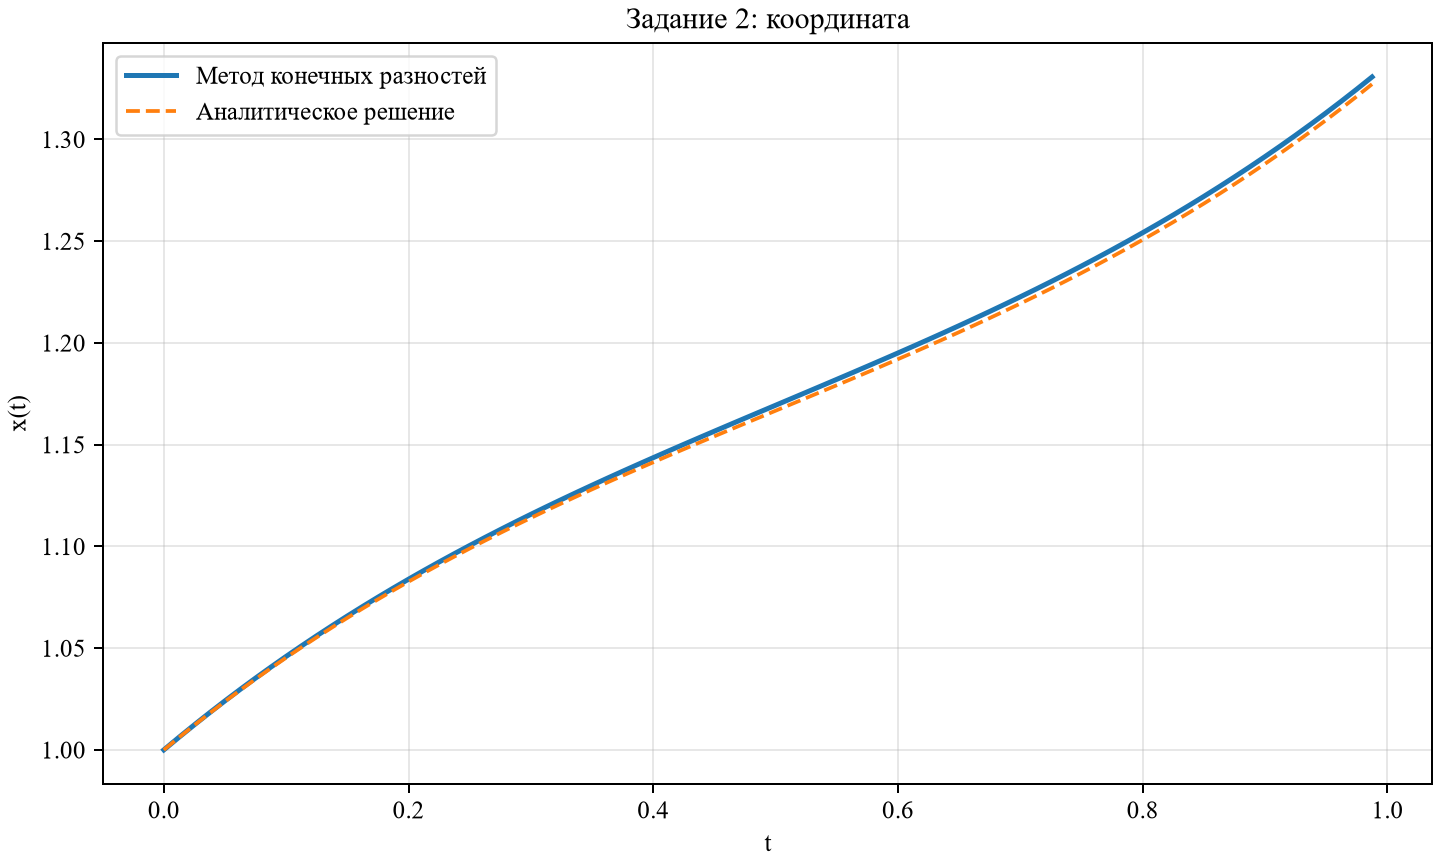
\includegraphics[width=0.78\textwidth]{task2_solution.png}
\caption{Численное и аналитическое решения задачи 2}
\end{figure}
\begin{figure}[H]
\centering
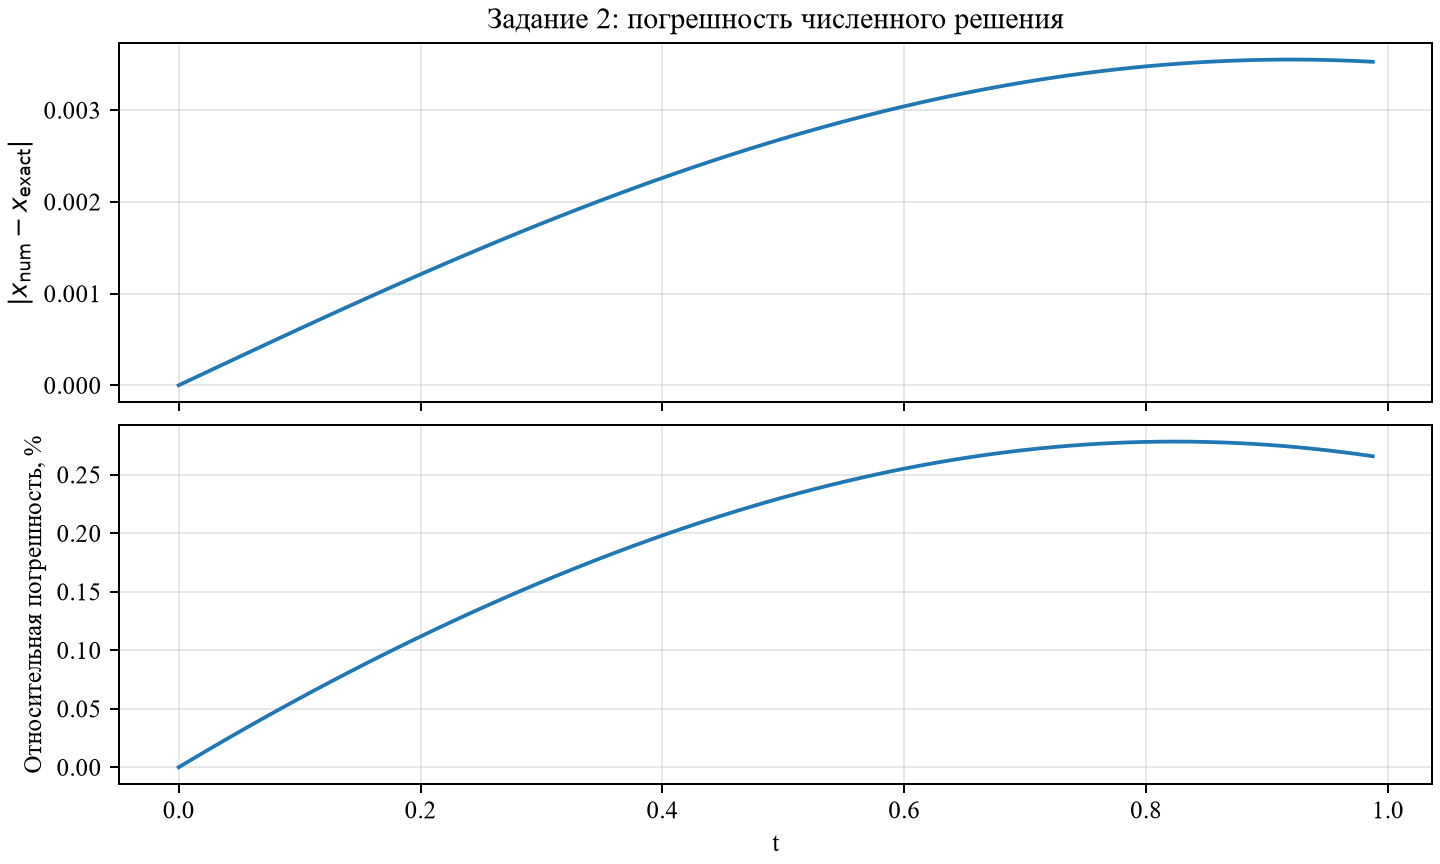
\includegraphics[width=0.82\textwidth]{task2_error.png}
\caption{Отклонение и относительная погрешность задачи 2}
\end{figure}

\subsection{Ответ на вопрос о характере движения}
Скорость численного решения вычислялась разностным дифференцированием, а
ускорение --- из исходного уравнения:
\[
x'(t)\approx \frac{d x_{\text{МКР}}}{dt},\qquad
x''(t)=\frac{t^2-x'(t)}{m}.
\]
Скорость сначала уменьшается, достигает минимума около \(t=0.5\), а затем
возрастает. Аналитически \(x''(t)=2t-1\): ускорение отрицательно при
\(t<0.5\), равно нулю при \(t=0.5\) и положительно после этой точки.
Следовательно, тело все время движется в положительном направлении, сначала
замедляясь, а затем ускоряясь.
\begin{figure}[H]
\centering
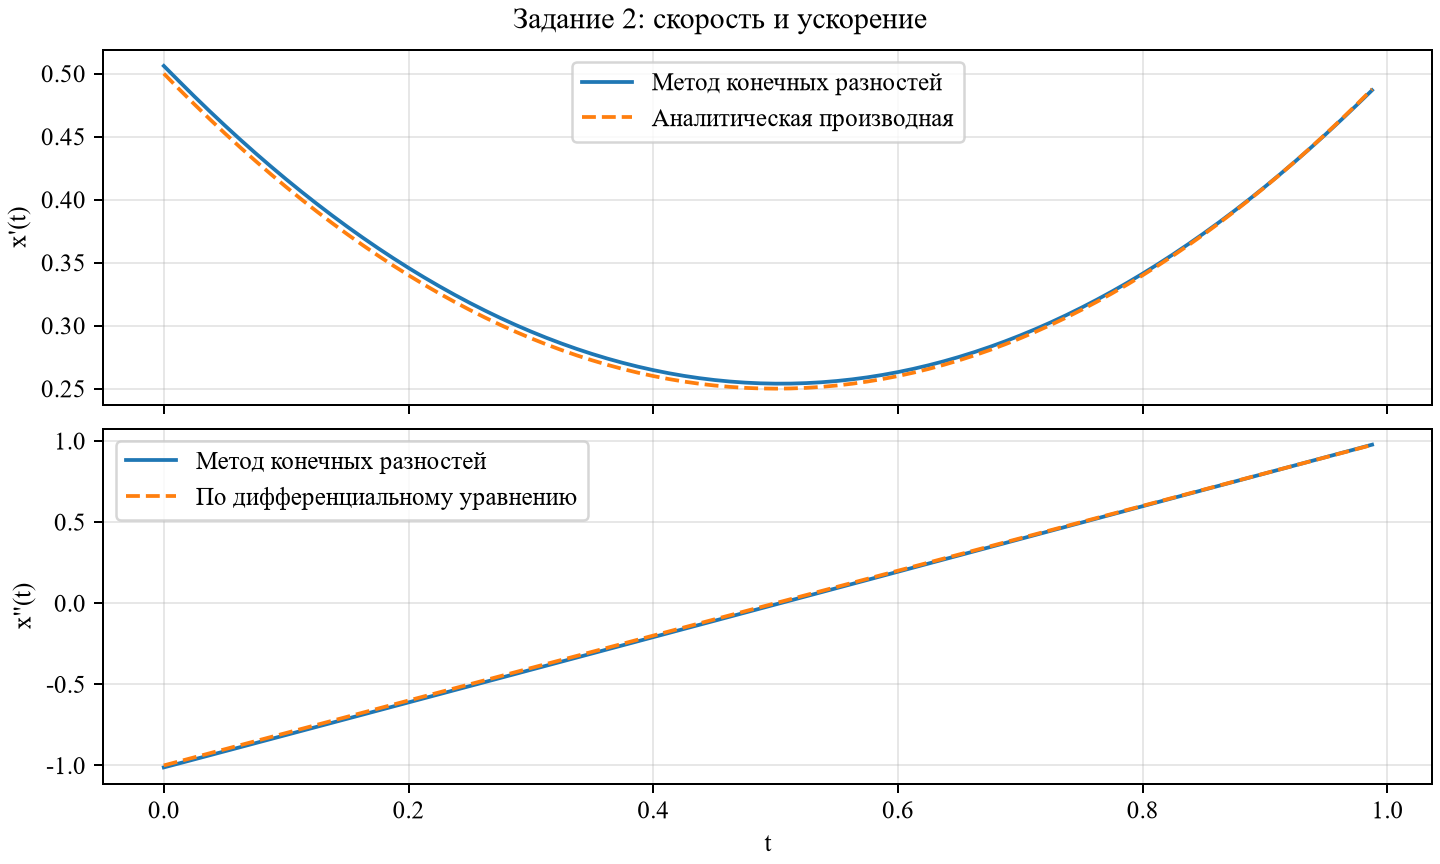
\includegraphics[width=0.82\textwidth]{task2_derivatives.png}
\caption{Скорость и ускорение в задаче 2}
\end{figure}

\section{Задание 3: двумерная задача Пуассона}
Рассмотрим квадрат \(0\le x,y\le1\), сетку \(N=40\) интервалов по каждому
направлению (\(h=0.025\)) и уравнение
\[
U_{xx}+U_{yy}=1,\qquad
U(x,0)=1,\quad U(0,y)=1.
\]
Уравнение задает двумерное скалярное поле с постоянным источником. На нижней и
левой сторонах заданы значения поля (условия Дирихле), а на верхней и правой
сторонах --- нормальные производные (условия Неймана). Решение показывает
распределение \(U(x,y)\) в квадратной области при этих источнике и граничных
условиях.
В условии для верхней стороны производная обозначена неоднозначно. В работе
принята стандартная постановка с нормальными производными на двух оставшихся
сторонах:
\[
U_y(x,1)=0.5,\qquad U_x(1,y)=0.5.
\]
Для внутренних узлов использована пятиточечная схема
\[
\frac{U_{i+1,j}-2U_{i,j}+U_{i-1,j}}{h^2}
+\frac{U_{i,j+1}-2U_{i,j}+U_{i,j-1}}{h^2}=1.
\]
На правой и верхней границах производные аппроксимированы односторонней
разностью первого порядка:
\[
\frac{U_{N,j}-U_{N-1,j}}{h}=0.5,\qquad
\frac{U_{i,N}-U_{i,N-1}}{h}=0.5.
\]
В угловом узле \((1,1)\) использовано среднее двух граничных уравнений
Неймана первого порядка, то есть
\[
\frac{(U_{N,N}-U_{N-1,N})+(U_{N,N}-U_{N,N-1})}{2h}=0.5.
\]
Полученная разреженная система линейных уравнений
решена методом разреженного прямого решения. На сетке получено
\(\min U\approx0.9804\), \(\max U\approx1.3921\),
\(U(0.5,0.5)\approx1.0271\).

\begin{figure}[H]
\centering
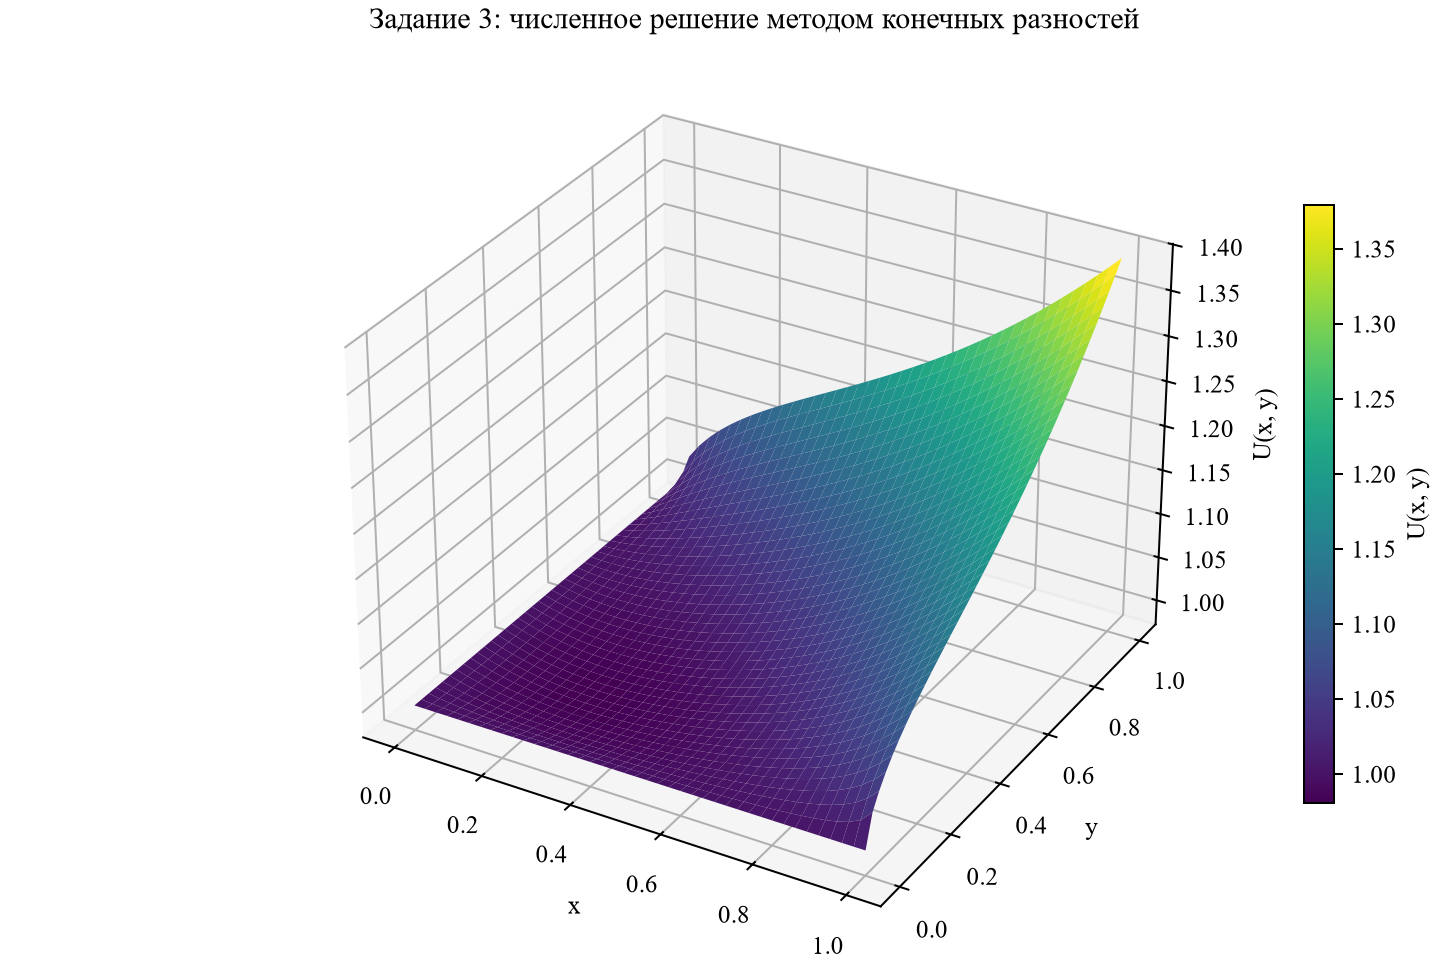
\includegraphics[width=0.82\textwidth]{task3_surface.png}
\caption{Поверхность численного решения задачи 3}
\end{figure}
\begin{figure}[H]
\centering
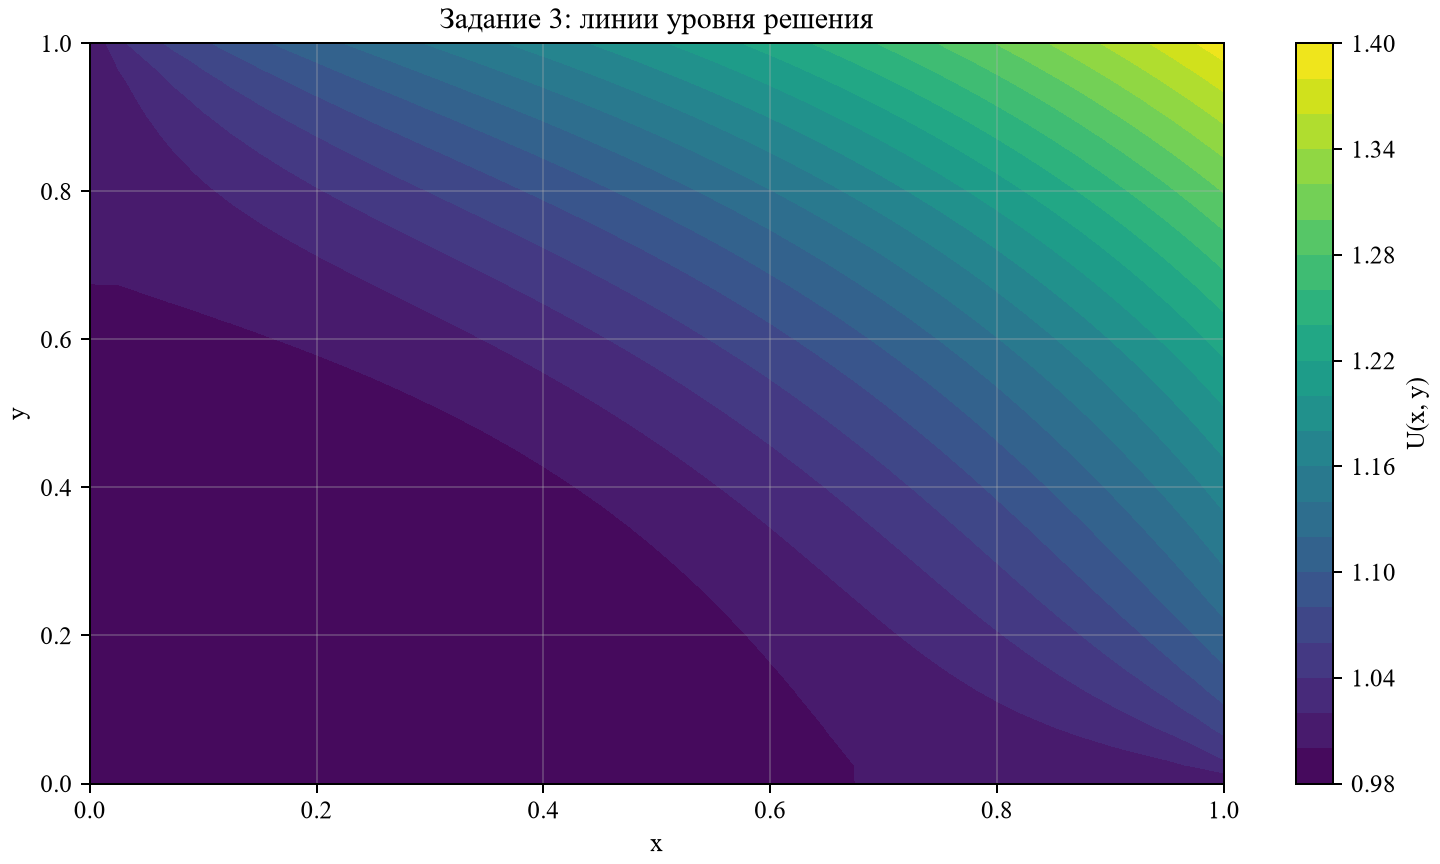
\includegraphics[width=0.75\textwidth]{task3_contour.png}
\caption{Линии уровня решения задачи 3}
\end{figure}

\section{Вывод}
В работе реализован МКР для двух задач Коши и двумерного уравнения Пуассона.
В первой задаче численное решение согласуется с точным квадратичным решением
с максимальной относительной погрешностью \(0.3064\%\). Во второй задаче для
правой части \(t^2\) погрешность не превышает \(0.2783\%\); движение на
интервале сначала замедленное, затем ускоренное. Для двумерной задачи построено
численное поле с граничными условиями Неймана, аппроксимированными разностями
первого порядка. Все графики и численные результаты воспроизводятся скриптом
Python, приложенным отдельно.

\end{document}
